\chapter{Modeling Microservices}\label{chapter:service_candidate}
In this chapter, various approaches to model microservices are identified from literature. Precisely, two distinct approaches are described in sections \ref{section:selection_by_use_case/use_case} and \ref{section:domain_driven_design/introduction} respectively. For each process, a detailed set of steps are formulated. Finally, in order to make it clear, an example problem domain is taken, which is then broken down into microservices using each of these two distinct models.
\section{Introduction}\label{section:service_candidate/introduction}
In the previous chapters, granularity and other quality attributes of a microservice were focussed. The qualitative as well as quantitative aspects of granularity were described. Additionally, various quality metrics were discussed to measure different quality attributes of a microservce. Moreover, a set of principle guidelines and basic metrics to qualify the microservices were also listed.\\
In addition to that, it is also equally important to agree on the process to identify the service candidates. In this chapter, the ways to model microservices will be discussed.
Basically, there are three basic approaches to identify service candidates: Top-down, bottom-up and meet-in-the-middle. \\
The top-down approach defines the process on the basis of the business model. At first, various models are designed to capture the overall system and architecture. Using the overall design, services are identified upfront in the analysis phase.\\
The next approach is bottom-up, which base its process on the existing architecture and existing application. The existing application is studied to identify the cohesion and consistency of the features provided by various components of the system. This information is used to aggregate the features and identify services in order to overcome the problems in the existing system.\\
Finally, the meet-in-the-middle approach is a hybrid approach of both top-down and bottom-up approaches. In this approach, the complete analysis of system as a whole is not performed upfront as the case of top-down approach. Where as, a set of priority areas are identified and used to analyse their business model resulting in a set of services. The services thus achieved are further analysed critically using bottom-up approach to identify problems. The problems are handled in next iterations where the same process as before is followed. The approach is continued for other areas of the system in the order of their priority.\cite{Pierre-Reldin:2007aa}\cite{Arsanjani:2004aa}\\
Considering the motive of the thesis, which is mainly concerned with green field development, top-down approaches will be taken into consideration. In this chapter, two different strategies discussed in literature which happen to be top-down approaches, will be explained in detail.

%-------------------------------------------------Modeling Using Use cases-------------------------------------------------
\section{Modeling Using Use cases}\label{section:selection_by_use_case/use_case}
A use case is an efficient as well as a fancy way of capturing requirements. Another technique of eliciting requirement is by features specification. However, the feature specification technique limits itself to answer only "what the system is intended to do". On the other hand, use case goes further and specifies "what the system does for any specific kind of user". In this way, it gives a way to specify and futhermore validate the expectation and concerns of stakeholders at the very early phase of software development. Undoubtedly for the same reason, it is not just a tool for requirement specification but an important software engineering technique which guides the software engineering cycle. Using use cases, the software can be developed to focus on the concerns that are valueable to the stakeholders and test accordingly.\cite{Ng:2004aa}
\\
It can be valueable to see the ways it has been defined.
\begin{shaded}Definition 1: \cite{Jacobson:1987aa} \end{shaded}
"A use case is a sequence of actions performed by the system to yield an observable result of value to a particular user." 
\\
\begin{shaded}Definition 2: \cite{Rumbaugh:1999aa}\end{shaded}
"A use case is a description of a set of sequences of actions, including variants, that a system performs that yield an observable result of value to an actor."

\subsection{Use case Refactoring}\label{section:selection_by_use_case/use_case_refactoring}
According to \cite{Jacobson:1987aa} it is not always intuitive to modularize use cases directly. As per the definitions provided in Section \ref{section:selection_by_use_case/use_case}, a use case consists of a number of ordered functions together to accomplish a certain goal. \cite{Jacobson:1987aa} defines these cohesive functionalites distributed across use cases as clusters. And the process of identifying the clusters scattered around the use cases, is the process of identifying services. \cite{Ng:2004aa} and \cite{Jacobson:2003aa} describes use case possibly consisting of various cross-cutting concerns. The papers use the term 'use case module' to define the cohesive set of tasks. Figure \ref{fig:selection_by_use_case/use_case_one} demonstrate the cross cutting functionalities needed by a use case in order to accomplish its goal. For example, the use case 'does A' has to perform separate functionalities on different domain entities X and Y. Similarly, the use case 'does B' needs to perform distinct functions on entities X, Y and Z.
\begin{figure}[H]
\begin{center}
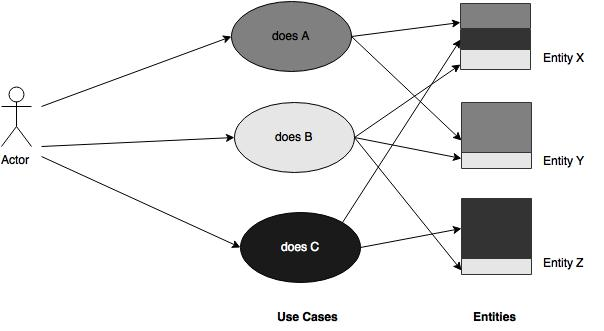
\includegraphics[width=0.8\textwidth]{figures/use-case-one}
\caption{Use cases with cross-cutting concerns \cite{Ng:2004aa}}
\label{fig:selection_by_use_case/use_case_one}
\end{center}
\end{figure}
This situation prompts for the analysis of the use cases for cross cutting tasks and refactoring them in order to map the cohesive functionalities and use cases. Refactoring helps to achieve the right level of abstraction and granularity by improving functionality cohesion as well as elimination of redundancy and finally promoting the reusablity. \cite{Doh:2007aa}
\\
Furthermore, the refactoring is assisted by various relationships in use case model to represent dependencies between use cases, which are include, generalization and extend. \cite{Ng:2004aa}
\\
\subsection{Process for Use Case Refactoring}\label{section:selection_by_use_case/process_for_use_case_refactoring}
In order to refactor the use cases and finally map use cases to the service, the papers \cite{Kim:2006aa}, \cite{Yun:2006aa} and \cite{Doh:2007aa} provide a comprehensive method. In this approach, use case models are first created and then refactored to create new set of use cases to accomplish high cohesion in functionality and loose coupling. This will ultimately create use cases supporting modularity. \cite{Fareghzadeh:2008aa} There are three distinct steps for service identification using service refactoring.
\begin{enumerate}
\item \textbf{TaskTree Generation}\\
In this step, the initial use case model created during domain analysis is used to create task trees for each distinct use case. The task trees provide sequence of individual tasks required to accomplish in order to achieve the goal of the use case.
\\
\item \textbf{Use Case Refactoring}\\
In this step, the task tree generated in the previous step is analysed. As already mentioned in the Section \ref{section:selection_by_use_case/use_case_refactoring}, the initial use case consists of various cross cutting functionalities which runs through large number of business entities. In order to minimize that, refactoring is performed. The detail rules are provided in Section \ref{section:selection_by_use_case/rules_for_use_case_refactoring}.
\\
\item \textbf{Service Identification}\\
The use cases achieved after refactoring have correct level of abstractions and granularity representing cohesive business functionality. The unit use cases thus achieved appreciate reuse of common functionality.  \cite{Doh:2007aa} Furthermore, the approach considers the concerns of stakeholders in terms of cohesive business functionalities to be represented by use cases.\cite{Fareghzadeh:2008aa} Additionally, the process also clarifies the dependencies between various use cases. Thus, the final use cases obtained can be directly maped to individual services.
\end{enumerate}
\\
\subsection{Rules for Use Case Refactoring}\label{section:selection_by_use_case/rules_for_use_case_refactoring}
The context is first defined before distinct rules are presented.
\\
\begin{shaded}Context 1 \end{shaded}
If U represents use case model of the application, $t_i$ represents any task of U and T being the set of tasks of U. Then, $\forall t_i \in T $, $t_i$ exists in the post-refactoring model U'. The refactoring of a use case model preserves the set of tasks.
\\
\begin{shaded}Context 2 \end{shaded}
A refactoring rule R is defined as a 3-tuple (Parameters, Preconditions, Postconditions). Parameters are the entities involved in the refactoring, precondition defines the condition which must be satisfied by the use case u in order for R to be applied in u. Postcondition defines the state of U after R is applied.
\\
The various refactoring rules are as listed below.
\\
\subsubsection{Decomposition Refactoring}\label{section:selection_by_use_case/guidelines_for_use_case_refactoring/decomposition_refactoring}
When the use case is complex and composed of various functionally independent tasks, the tasks can be ejected out of the task tree of the use case and represented as a new use case. The Table \ref{tab:selection_by_use_case/guidelines_for_use_case_refactoring/decomposition_rule} shows the decomposition rule in detail.
\begin{table}[H]
  \centering
  \begin{adjustbox}{max width=\textwidth}
  \begin{tabular}{*{14}{|c}|}%%{|c|l|}
  \hline
  Parameters & 
                    \begin{tabular}{ll}
                    \multirow{3}{*}
                    &u: a use case to be decomposed\\
                    &t: represents task tree of u \\
                    &t': a subtask tree of t\\
                    \end{tabular}\\
                    \hline
   Preconditions  & t' is functionally independent of u \\
                    \hline
   Postconditions &
                    \begin{tabular}{ll}
                    \multirow{2}{*}
                    &1. new use case u' containing task tree t' is generated \\
                    &2. a dependency is created between u and u'\\
                    \end{tabular}\\
                    \hline
\end{tabular}
\end{adjustbox}
  \caption{Decomposition Rule}
  \label{tab:selection_by_use_case/guidelines_for_use_case_refactoring/decomposition_rule}
\end{table}
\\

\subsubsection{Equivalence Refactoring}\label{section:selection_by_use_case/guidelines_for_use_case_refactoring/equivalence_refactoring}
If the two use cases share their tasks in the task tree, we can conclude that they are equivalent and redundant in the use case model. The Table \ref{tab:selection_by_use_case/guidelines_for_use_case_refactoring/equivalence_rule} shows the rule for the refactoring.
\begin{table}[H]
  \centering
  \begin{adjustbox}{max width=\textwidth}
  \begin{tabular}{*{14}{|c}|}%%{|c|l|}
  \hline
  Parameters &  $u_1$ , $u_2$: two distinct use cases\\
                    \hline
   Preconditions  & the task trees of $u_1$ and $u_2$ have same behavior \\
                    \hline
   Postconditions &
                    \begin{tabular}{ll}
                    \multirow{3}{*}
                    &1. $u_2$ is replaced by $u_1$ \\
                    &2. all the relationship of $u_2$ are fulfilled by $u_1$\\
                    &3. $u_2$ has no relationship with any other use cases\\
                    \end{tabular}\\
                    \hline
\end{tabular}
\end{adjustbox}
  \caption{Equivalence Rule}
  \label{tab:selection_by_use_case/guidelines_for_use_case_refactoring/equivalence_rule}
\end{table}
\\

\subsubsection{Composition Refactoring}\label{section:selection_by_use_case/guidelines_for_use_case_refactoring/composition_refactoring}
When there are two or more small-grained use cases such that they have related tasks, the use cases can be represented by a composite unit use case.

\begin{table}[H]
  \centering
  \begin{adjustbox}{max width=\textwidth}
  \begin{tabular}{*{14}{|c}|}%%{|c|l|}
  \hline
  Parameters & 
                 \begin{tabular}{ll}
                    \multirow{3}{*}
                    & $u_1$, $u_2$: the fine grained use cases\\
                    & $t_1$, $t_2$: the task trees of $u_1$ and $u_2$ respectively\\
                    \end{tabular}\\
                    \hline
   Precondition     & $t_1$ and $t_2$ are functionally related.\\
                    \hline
   Postconditions &
                    \begin{tabular}{ll}
                    \multirow{3}{*}
                    & 1. $u_1$ and $u_2$ are merged to a new unit use case u \\
                    & 2. u has new task tree given by $t_1 \cup t_2 $\\
                    & 3. the dependencies of $u_1$ and $u_2$ are handled by u\\ 
                    & 4. $u_1$ and $u_2$ are deleted along with their task trees $t_1$ and $t_2$\\
                    \end{tabular}\\
                    \hline
\end{tabular}
\end{adjustbox}
  \caption{Composition Rule}
  \label{tab:selection_by_use_case/guidelines_for_use_case_refactoring/composition_rule}
\end{table}
\\

\subsubsection{Generalization Refactoring}\label{section:selection_by_use_case/guidelines_for_use_case_refactoring/generalization_refactoring}
When multiple use cases share some volume of dependent set of tasks in their task trees, it can be implied that the common tasks set can be represented by a new use case. The Table \ref{tab:selection_by_use_case/guidelines_for_use_case_refactoring/generalization_rule} provides the specific of the rule.
\begin{table}[H]
  \centering
  \begin{adjustbox}{max width=\textwidth}
  \begin{tabular}{*{14}{|c}|}%%{|c|l|}
  \hline
  Parameters & 
                 \begin{tabular}{ll}
                    \multirow{2}{*}
                    & $u_1$ , $u_2$: two distinct use cases\\
                    & $t_1$ , $t_2$: task trees of $u_1$ and $u_2$ respectively\\
                    \end{tabular}\\
                    \hline
   Precondition     & $t_1$ and $t_2$ share a common set of task $t= \{ x_1, x_2...x_n \} $\\
                    \hline
   Postconditions &
                    \begin{tabular}{ll}
                    \multirow{5}{*}
                    & 1. a new use case u is created using task tree $t= \{x_1, x_2...x_n \} $ \\
                    & 2. relationship between u with $u_1$  and between u with $u_2$ is created\\
                    & 3. the task tree $t= \{ x_1, x_2...x_n \} $ is removed from task tree of both $u_1$ and $u_2$\\
                    & 4. the common relationship of both $u_1$ and $u_2$ are handled by u and \\ 
                    & removed from them\\
                    \end{tabular}\\
                    \hline
\end{tabular}
\end{adjustbox}
  \caption{Generalization Rule}
  \label{tab:selection_by_use_case/guidelines_for_use_case_refactoring/generalization_rule}
\end{table}
\\


\subsubsection{Merge Refactoring}\label{section:selection_by_use_case/guidelines_for_use_case_refactoring/merge_refactoring}
When a use case is just specific for another use case and the use case is only the consumer for it, the two use cases can be merged into one.
\begin{table}[H]
  \centering
  \begin{adjustbox}{max width=\textwidth}
  \begin{tabular}{*{14}{|c}|}%%{|c|l|}
  \hline
  Parameters & 
                 \begin{tabular}{ll}
                    \multirow{3}{*}
                    & u, u': the use cases\\
                    & r defines the dependency of u with u'\\
                    & t, t': the task trees of u and u' respectively\\
                    \end{tabular}\\
                    \hline
   Precondition     & there is no dependency of other use cases with u' except u\\
                    \hline
   Postconditions &
                    \begin{tabular}{ll}
                    \multirow{3}{*}
                    & 1. u' is merged to u \\
                    & 2. u has new task tree given by $t \cup t' $\\
                    & 3. r is removed\\
                    \end{tabular}\\
                    \hline
\end{tabular}
\end{adjustbox}
  \caption{Merge Rule}
  \label{tab:selection_by_use_case/guidelines_for_use_case_refactoring/merge_rule}
\end{table}
\\

\subsubsection{Deletion Refactoring}\label{section:selection_by_use_case/guidelines_for_use_case_refactoring/deletion_refactoring}
When a use case is defined but no relationship can be agreed with other use cases or actors then it can be referred that the use case represent redundant set of tasks which has already been defined by other use cases.
\begin{table}[H]
  \centering
  \begin{adjustbox}{max width=\textwidth}
  \begin{tabular}{*{14}{|c}|}%%{|c|l|}
  \hline
  Parameters      & u: a distinct use case\\
                    \hline
   Precondition     & the use case u has no relationship with any other use cases and actors\\
                    \hline
   Postconditions   & the use case u is deleted\\
                    \hline
\end{tabular}
\end{adjustbox}
  \caption{Deletion Rule}
  \label{tab:selection_by_use_case/guidelines_for_use_case_refactoring/deletion_rule}
\end{table}
\\

\subsection{Example Scenario}\label{section:selection_by_use_case/refactoring_example}
In this section, a case study will be taken as an example. The case study will be modeled using use case. Finally, the use case will be refactored using the rules listed by \ref{section:selection_by_use_case/rules_for_use_case_refactoring}.
\\
\begin{shaded} Case Study \end{shaded}
The case study is about an international hotel named 'XYZ' which has branches in various locations. In each location, it offers rooms with varying facilities as well as prices. In order to make it easy for customers to find room irrespective of the location of customer, it is planning to offer an online room booking application. Using this application, any registered customer can search for a room according to his/her requirement in any location. When he/she is satisfied, can book the room online as well. The customer will be sent notification by email regarding booking. At present, the payment will be accepted in person, only after the customer gets into the respective branch. Finally, if the customer wants to cancel the room, he/she can do online anytime. The customer will also be notified by e-mail to confirm the cancelation of booking. It is an initial case study so only priority cases and conditions are considered here.
\\
\\
The remaining part of this section presents the steps to indentify the services using use case refactoring following the process defined in Section \ref{section:selection_by_use_case/process_for_use_case_refactoring} and rules presented in the Section \ref{section:selection_by_use_case/rules_for_use_case_refactoring}
\\
\\
\textbf{\underline{Step 1:}}
\\
\\
The initial analysis of the case study will produce use case model as shown by figure \ref{fig:selection_by_use_case/use_case_two}.

\begin{figure}[H]
\begin{center}
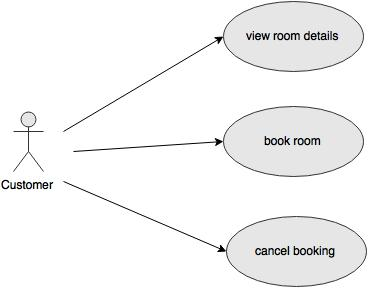
\includegraphics[width=0.5\textwidth]{figures/use-case-two}
\caption{Initial Use Case Model for Online Room Booking Application}
\label{fig:selection_by_use_case/use_case_two}
\end{center}
\end{figure}
\\
\\
\textbf{\underline{Step 2:}}
\\
\\
For each initial use case, task trees are generated which are needed to accomplish the desired functionality of respective use cases.
\\
\begin{table}[H]
  \centering
  \begin{adjustbox}{max width=\textwidth}
  \begin{tabular}{*{14}{|c}|}%%{|c|l|}
  \hline
  \textbf{Use Case} & \textbf{Task Tree} \\
  \hline
  book room & 
                 \begin{tabular}{ll}
                    \multirow{9}{*}
                    & customer enters access credentials\\
                    & system validates the credentials\\
                    & customer enters location and time details for booking\\
                    & system fetch the details of empty rooms according to the data provided\\
                    & system displays the details in muliple pages\\
                    & customer choose the room and submits for booking\\
                    & system generates a booking number\\
                    & System updates the room\\
                    & system sends notification to the customer regarding booking\\
                    \end{tabular}\\
                    \hline
   cancel booking   &
                    \begin{tabular}{ll}
                    \multirow{7}{*}
                    & customer enters access credentials\\
                    & system validates the credentials\\
                    & customer enters the booking number\\
                    & system validates the booking number\\
                    & customer cancels the booking\\
                    & system updates the room\\
                    & system sends notification to the customer regarding cancelation\\
                    \end{tabular}\\
                    \hline
   view room details &
                    \begin{tabular}{ll}
                    \multirow{5}{*}
                    & customer enters access credentials\\
                    & system validate the credentials\\
                    & customer enter location and time\\
                    & system fetch the details of empty rooms according to the data provided\\
                    & system display the details in multiple pages\\
                    \end{tabular}\\
                    \hline
\end{tabular}
\end{adjustbox}
  \caption{Task Trees for Initial Use Cases}
  \label{tab:selection_by_use_case/guidelines_for_use_case_refactoring/initial_task_tree}
\end{table}
\\
\textbf{\underline{Step 3:}}
\\
The initial task trees created for each use case at Step 2 is analysed. There are quite a few set of tasks which are functionally independent of the use case goal and also few tasks which are common in more use use cases. The following Table \ref{tab:selection_by_use_case/guidelines_for_use_case_refactoring/common_and_independent_tasks} lists those tasks from the tasks trees \ref{tab:selection_by_use_case/guidelines_for_use_case_refactoring/initial_task_tree} which are either functionally independent from their corresponding use cases or common in more use cases.
\\
\begin{table}[H]
  \centering
  \begin{adjustbox}{max width=\textwidth}
  \begin{tabular}{*{14}{|c}|}%%{|c|l|}
  \hline
  \textbf{Tasks Type} & \textbf{Tasks} \\
  \hline
  Independent Tasks & 
                 \begin{tabular}{ll}
                    \multirow{9}{*}
                    & system validates the credentials\\
                    & system fetch the details of empty rooms according to the data provided\\
                    & system generates a booking number\\
                    & system validates the booking number\\
                    & system updates the room\\
                    & system sends notification to the customer
                    \end{tabular}\\
                    \hline
   Common Tasks   &
                \begin{tabular}{ll}
                    \multirow{9}{*}
                    & system validates the credentials\\
                    & system fetch the details of empty rooms according to the data provided\\
                    & system updates the room\\
                    & system sends notification to the customer
                    \end{tabular}\\
                    \hline
\end{tabular}
\end{adjustbox}
  \caption{Common and Independent Tasks}
  \label{tab:selection_by_use_case/guidelines_for_use_case_refactoring/common_and_independent_tasks}
\end{table}
\\
Now, for independent tasks the docomposition rule explained by \ref{tab:selection_by_use_case/guidelines_for_use_case_refactoring/decomposition_rule} can be applied and for common tasks, the generalization rule given by \ref{tab:selection_by_use_case/guidelines_for_use_case_refactoring/generalization_rule} can be applied. The use cases obtained after applying these rules is shown by the figure \ref{fig:selection_by_use_case/use_case_three}
\\
\begin{figure}[H]
\begin{center}
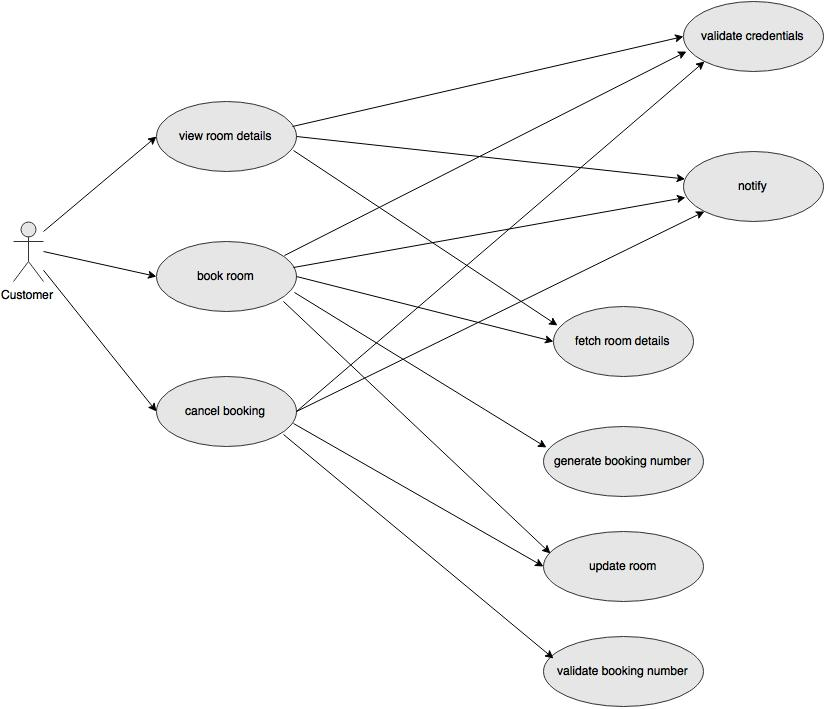
\includegraphics[width=0.7\textwidth]{figures/use-case-three}
\caption{Use Case Model after applying Decomposition and Generalization rules}
\label{fig:selection_by_use_case/use_case_three}
\end{center}
\end{figure}
\\
\textbf{\underline{Step 4:}}
\\
The use case model \ref{fig:selection_by_use_case/use_case_three} obtained in Step 3 is analysed again for further refactoring. It can seen that the use cases 'fetch room details' and 'update room' are fine grained and related to same business model 'Room'. Similarly, the use cases 'generate booking number' and 'validate booking number' are related to business entity 'Booking Number'. The composition rule explained by \ref{tab:selection_by_use_case/guidelines_for_use_case_refactoring/composition_rule} can be applied to these use cases, which will then result in use case model shown by figure \ref{fig:selection_by_use_case/use_case_four}
\\
\begin{figure}[H]
\begin{center}
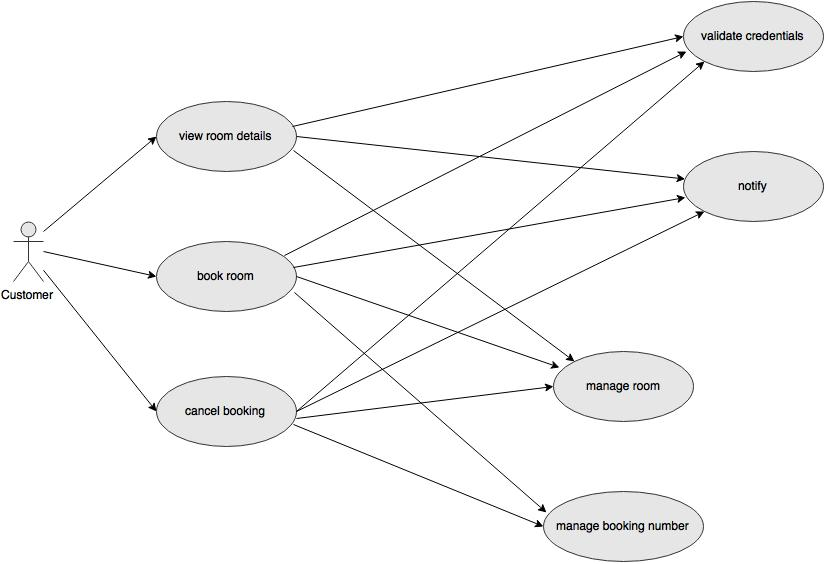
\includegraphics[width=0.8\textwidth]{figures/use-case-four}
\caption{Use Case Model after applying Composition rule}
\label{fig:selection_by_use_case/use_case_four}
\end{center}
\end{figure}
\\
\textbf{\underline{Step 5:}}
\\
Finally, the use case obtained in step 4 is used to identify the service candidates. The final use cases obtained in Step 4 have appropriate level of granularity and cohesive functionalities to be identified as individual services. Most importantly, the refactoring has now separated the cross cutting concerns in terms of various reusable fine grained use cases as shown by the figure. If we compare the the final use case model \ref{fig:selection_by_use_case/use_case_five} with respect to Figure \ref{fig:selection_by_use_case/use_case_one}, then it can be implied that the functionalities operating on business entities as well as the business logic serving the candidate concerns are separated and represented by individual use cases. So, the each use case can be mapped to individual services. The services are as listed in the bottom of the Figure \ref{fig:selection_by_use_case/use_case_five}.
\\
\begin{figure}[H]
\begin{center}
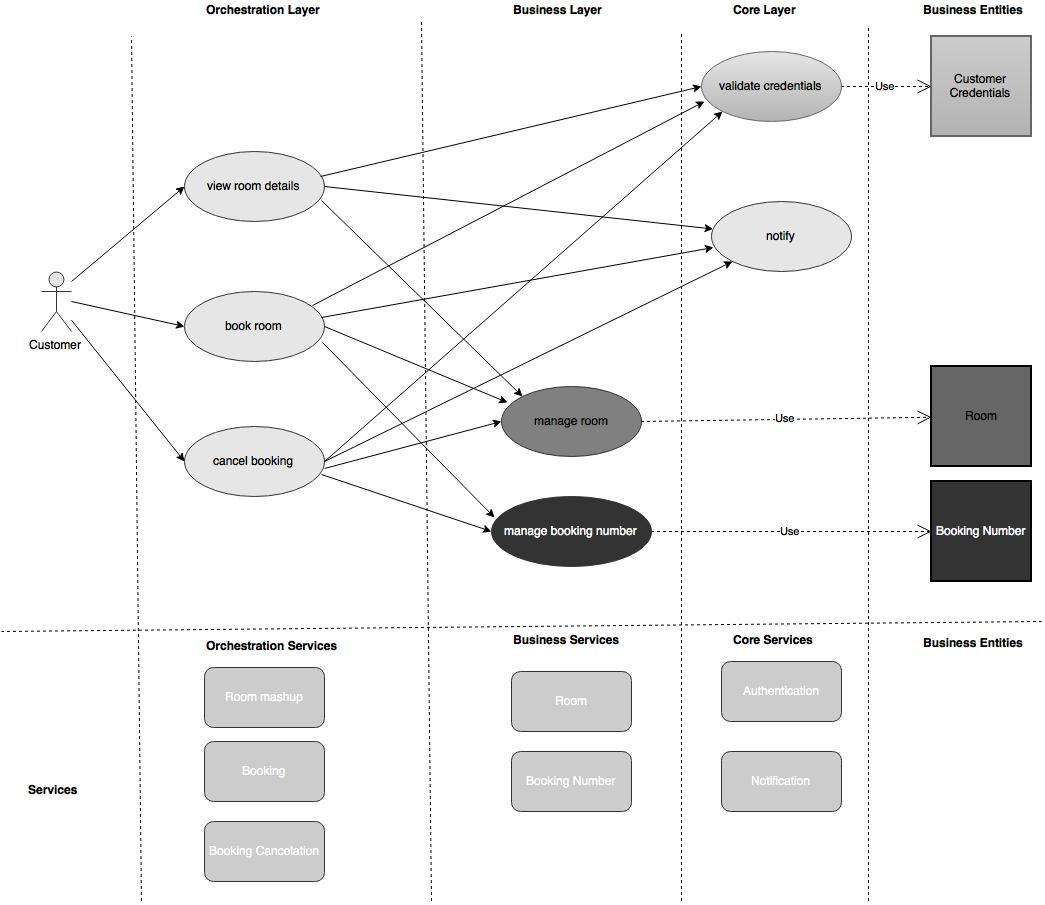
\includegraphics[width=0.8\textwidth]{figures/use-case-five}
\caption{Use Case Model for identification of service candidates}
\label{fig:selection_by_use_case/use_case_five}
\end{center}
\end{figure}
\\
\textbf{Microservices Layers}\\
The services obtained as shown in the Figure \ref{fig:selection_by_use_case/use_case_five} from the refactoring process, creates various levels of abstractions. The levels of abstractions represents different level of functionality. The services at the bottom layer are core services which serve many higher level services. These services are not dependent on any other services. 'Notification' and 'Authentication' are core services obtained from refactoring. The layer above the core layer is business layer. The business service can either have entity services, which control some related business entities or can have task services which provides some specific business logic to higher level services. 'Room' and 'Booking Number' are the entity services obtained from refactoring. Finally, the top layer is mashup layer which contains high level business logic and collaborates with business services as well as core services. 'Room mashup' , 'Booking' and 'Booking Cancelation' are orchestration layer services obtained. The individual services as well as their respective layers are shown in Figure \ref{fig:selection_by_use_case/use_case_five}. \cite{Fareghzadeh:2008aa}\cite{Emig:2015aa}\cite{Zimmermann:2005aa}

%-------------------------------------------------Domain Driven Design-------------------------------------------------
\section{Modeling using Domain Driven Design}\label{section:domain_driven_design/introduction}
Understanding the problem space can be a very useful way to design software. The common way to understand the problem and communicate them is by using various design models. The design models are the abstraction as well as representation of the problem space. However, when the abstractions are created, there are chances that important concepts or data are ignored or misread. This will highly impact the quality of software produced. The software thus developed may not reflect the real world situation or problem entirely.
\\
Domain Driven Design provides a way to represent the real world problem space so that all the important concepts and data from real world remains intact in the model. The domain model thus captured respects the differences as well as the agreement in the concepts across various parts of the problem space. Moreover, it also provides a way to divide the problem space into manageable independent partitions and makes it easy for developers as well as stakeholders to focus on the area of concern and be more agile. Finally, the domain models act as the understandable and common view of the business for both domain experts as well as the developers. This will make sure that the software developed using domain driven design will comply with business need.\cite{Evans:2003aa}\cite{Vernon:2013aa}
\\

\subsection{Process to implement Domain Driven Design}\label{section:domain_driven_design/process_to_domain_driven_design}
There are three basic parts to implement domain driven design:
\begin{enumerate}
\item{Ubiquitous Language}
\item{Strategical Design}
\item{Tactical Design}
\end{enumerate}
\\
As the focus is to describe the process of modeling microservices, only the first two parts are relevant and will be focused in the later part of this chapter.
\subsubsection{Ubiquitous Language}\label{section:domain_driven_design/process_to_domain_driven_design/ubiquitous_language}
Ubiquitous Language is a common language agreed among domain experts and developers in a team. It is important to have a common understanding about the concepts of a business which is being developed and ubiquitous language is the way to assure that. Domain Experts understand the domain in terms of their own jargon and concept. It is difficult for a developer to understand them. Usually, developers translates those jargons into the terms they understand easily, during design and implementation. However along the way of translation, major domain concepts can get lost and the immediate value of the resulting solution might decrease tremendously. In order to prevent creation of such low valued solution, there should be a an approach to define common vocabularies and concepts understood by all domain experts as well as the developers. These common vocabularies and concepts make the core of the ubiquitous language.\cite{Evans:2003aa}\cite{Vernon:2013aa}
\\
Along with the common vocabulary and concepts, domain models provide backbone to create ubiquitous language. The models represents not only artifacts but also functionalities, rules and strategies. It is a way to express the common understanding in a visual form, providing an easy tool to comprehend.\cite{Evans:2003aa}\cite{Fowler:2006aa} According to \cite{Fowler:2003aa}, domain model should not be confused with data model which represents the business in datacentric view however each domain object should contain data as well as logic closely related to the data contained. Domain models are conceptual models rather than software artifacts but can be effectively visualized using \acrshort{UML}.\cite{Scott:2001aa}

\begin{figure}[H]
\begin{center}
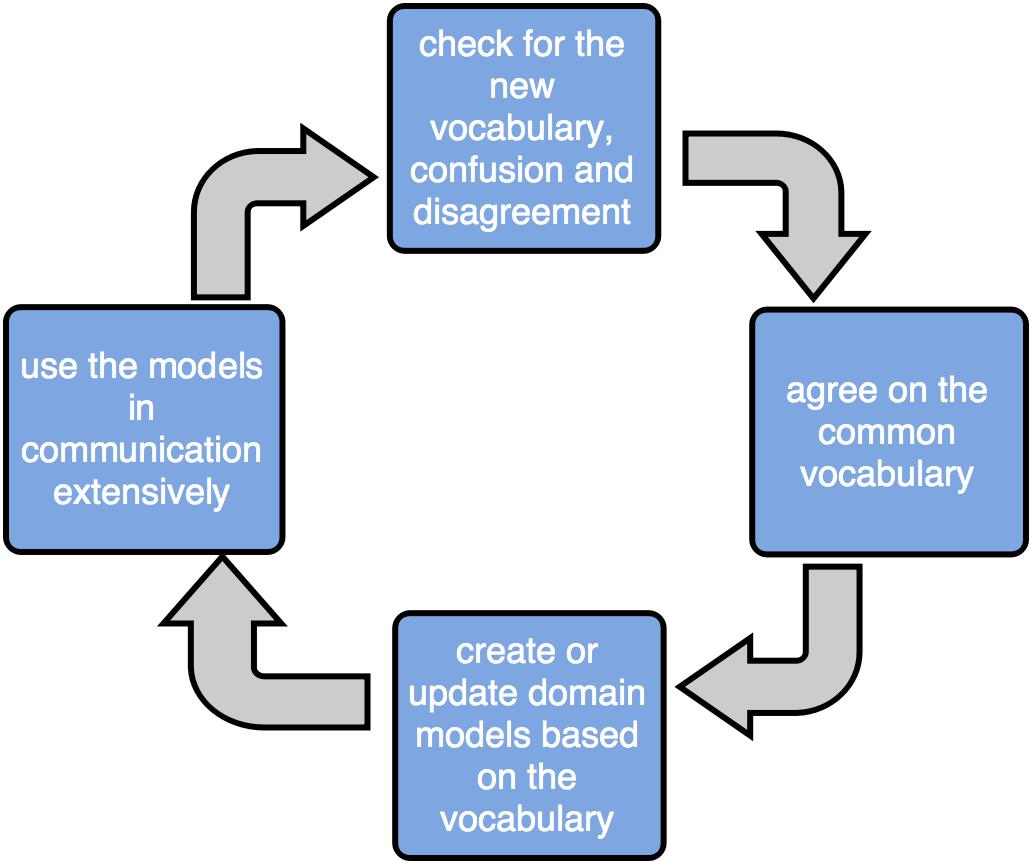
\includegraphics[width=0.8\textwidth]{figures/domain-driven-design-one}
\caption{Process to define Ubiquitous Language \cite{Evans:2003aa}}
\label{fig:domain_driven_design/ubiquitous_language_process}
\end{center}
\end{figure}
\\
The Figure \ref{fig:domain_driven_design/ubiquitous_language_process} visualizes the process of discovering the ubiquitous language in any domain. It is not a discretely timed phenomenon but a continous procedure with various phases occuring in a cycle throughout the development.
\\
On arrival of any new term, concept or any confusion, the contextual meaning of those terms are made clear before adding to the domain vocabulary. Next, the vocabularies and concepts are used to create various domain models following \acrshort{UML}. The domain models and various vocabularies form the common laguage among domain experts and developers within the team. It is very important to use only domain vocabularies for communication and understanding which will not only help to reflect the hidden domain concepts in the implementation but also create opportunities to find new vocabularies or refine existing ones in the event of confusion and disagreement.\cite{Evans:2003aa}
\\
Thus, the common vocabulary and domain models form the core of the ubiquitous language and the only way of coming up with the better one is by applying it in communication extensively. Ubiquitous language is not just a collection or documentation of terms but is the approach of communication within a domain.
\\
\subsubsection{Strategical Design}\label{section:domain_driven_design/process_to_domain_driven_design/strategical_design}
When applying model-driven approach to an entire enterprise, the domain models get too large and complicated. It becomes difficult to analyse and understand all at once. Furthermore, it gets worse as the system gets bigger and complex. The strategical design provides a way to divide the entire domain models into small,manageable and interoperable parts which can work together with low dependency in order to reflect the functionalities of the entire domain. The goal is to divide the system into modular parts which can be easily integrated. Additionally, the all-cohesive unified domain models of the entire enterprise cannot reflect differences in contextual vocabularies and concepts. \cite{Fowler:2014ab}\cite{Evans:2003aa}\cite{Vernon:2013aa}
\\
The strategical design specifies two major steps which are crucial in identifying microservices.
\\
\begin{shaded}Step 1: Divide problem domain into subdomains \end{shaded} \label{section:domain_driven_design/process_to_domain_driven_design/strategical_design/step_1}
\\
The domain represents the problem being solved by the software. The domain can be divided into various sub-domains based on the organizational structure of the enterprise, each sub-domain responsible for certain area of the problem. The \cite{Engels:2015aa} provides a comprehensive set of steps to identify sub-domains.
\begin{enumerate}
\item \textbf{Identify core business functionalities and map them into domain:} \\
A core business functionality represents the direct business capability which holds high importance and should be provided by the enterprise in order for it to succeed. For example, for any general e-commerce enterprise, the core focus will on the high amount orders being received from the customers and maintain the inventory to fulfil the orders. So, for those kind of e-commerce enterprises, 'Order Management' and 'Inventory Management' will be the some of the core domains.
\\
\item \textbf{Identify generic and supporting subdomains:} \\
The business capabilities which are viable for the success of business but not represent the specialization of the enterprise falls into supporting subdomains. The supporting subdomain does not require the enterprise to excel in these areas. Additionally, if the functionalities are not specific to the business but in a way support the business functionalities, then these are covered by generic subdomains. For example: for an e-commerce enterprise, 'Payment Management' can be a supporting subdomain whereas 'Reporting' and 'Authentication' can be generic subdomains.\cite{Vernon:2013aa}
\\
\item \textbf{Divide existing subdomains having multiple independent strategies:}\\
The subdomains found from earlier steps are analyzed to check if there are mutually independent strategies to handle the same functionality. The subdomain can then be further divided into multiple subdomains along the dimension of strategies. For example: the 'Payment Managment' subdomain discovered in earlier step can have different way of handling online payment depending upon the provider such as bank or paypal etc. In that case 'Payment Management' can be further divided into 'Bank Payment Management' and 'Paypal Payment Management'.
\end{enumerate}
\\
\begin{shaded}Step 2: Indentify bounded contexts\end{shaded} \label{section:domain_driven_design/process_to_domain_driven_design/strategical_design/step_2}
\\
As stated earlier of this section, the attempt to use a single set of domain models for the entire enterprise adds complexity for understanding and analysis. There is another important reason supporting the issue which is called unification of the domain models. Unification represents internal consistency of the terms and concepts described by the domain models. It is not always possible to have consistent meaning of terms without any contradictory rules throughout the enterprise. The identification of the logically consistent and inconsistent domain model creates a boundary around domain model. This boundary will bind all the terms which share consistent logic from those which are different so that there is clear understanding of the concept inside the boundary without any confusion. The shared context inside the boundary is defined as the bounded context.
\\
\textbf{Definition 1:} \label{bounded_context_definition_1}
\\
" A Bounded Context delimits the applicability of a particular model so that team members hava a clear and shared understanding of what has to be consistent and how it relates to other contexts. A bounded context has specific functionality and explicitly defines boundary around team organization, code bases and database schemas."\cite{Evans:2003aa}
\\
\textbf{Definition 2:} \label{bounded_context_definition_2}
\\
" A Bounded Context is an explicit boundary within which a domain model exists. Inside the boundary all terms and phrases of the Ubiquitous Language have specific meaning, and the model reflects the Language with exactness." \cite{Vernon:2013aa}
\\
\textbf{Definition 3:} \label{bounded_context_definition_3}
" A Bounded Context is a specific responsibility enforced by explicit boundaries." \cite{Mike:2012aa}
\\
Thus, the idea of bounded context provide the applicability of the ubiquitous language inside its boundary performing a specific responsibility. Outside the bounded contexts, teams have different ubiquitous language with different terms, concepts, meanings and functionalities. Apart from identifying independent and specific responsibilities inside a subdomain in order to identify bounded contexts, there are some general rules which can be considered as well.
\begin{enumerate}
\item \textbf{Assign individual bounded context to the subdomains identified in Step 1}
\\
Each subdomains have distinct functionalities and complete set of independent domain models to accomplish the functionalities. Thus, one to one mapping of subdomain and bounded context is possible ideally whereas in real cases, it may not be always possible which can be tackled using the rules discussed in further steps. For example: Order Management and Inventory Management can be two distinct bounded context each with own consistent ubiquitous language. \cite{Fowler:2014ab}\cite{Gorodinski:2013aa}
\\
\item \textbf{Identify polysemes}
\\
Polysemes are the terms which have different meaning in separate contexts. If the example of the generic subdomain 'Authentication' is taken. It can have an model 'Account' however the same model can refer to multiple concept such as social account identified by e-mail or registered account identified by unique username. The handling of these two separate concepts is also different which clearly suggests two separate context for each within 'Authentication' subdomain. Additionally, there can be polysemes in two separate domains as well. For example: there is also 'Account' model to identify bank account in the subdomain 'Bank Payment Management'. The identification of polysemes is vital to create clear boundary around which the concept and handling of such polysemes are consistent. \cite{Fowler:2014ab}
\\
\item \textbf{Identify independent generic functionality supporting the subdomain}
\\
There can be a necessity of independent technical functionality required to accomplish the business functionality of the subdomain only. Since it is only required by the particular subdomain, the functionality cannot be nominated as a generic subdomain. In such a case, the independent technical functionality can be realized as a separate bounded context. For example, in the subdomain 'Inventory Management', the functionality of full-text search can be assigned a separate bounded context as it is independent.\cite{Gorodinski:2013aa}
\end{enumerate}
\\
\subsection{Microservices and Bounded Context}\label{section:domain_driven_design/microservices_and_bounded_context}
Analyzing various definitions of microservices provided in Section \ref{section:context/microservices_architecture_style}, a list of important features with respect to specific category such as granularity or quality was compiled in the table \ref{tab:context/microservices_architecture_style/keywords_extracted_from_various_definitions_of_microservice}. In addition to the definitions of bounded context provided in Section \ref{bounded_context_definition_1}, the following definition of Domain Driven Design can be helpful to find analogy between a microservice and a bounded context.
\begin{shaded}Definition: Domain Driven Design\end{shaded}
"Domain Driven Design is about explaining what your company does in isolated parts, in performing these specific parts and you can have a dedicated team to do this stuff, and you can have different tools for different teams." \cite{Riggins:2015aa}
\\
\\
Using Table \ref{tab:context/microservices_architecture_style/keywords_extracted_from_various_definitions_of_microservice} and concepts extracted from various definitions of bounded context as well as Domain Driven Design provided, the Table \ref{tab:domain_driven_design/microservices_and_bounded_context/Analogy_of_Microservice_and_Bounded_Context} is generated. 
\\
\begin{table}[h!]
  \centering
  \begin{adjustbox}{max width=\textwidth}
  \begin{tabular}{*{14}{|c}|}%%{|c|c|}
  \hline
  \# & Expected features of a microservice  & Fulfilled by Bounded Context\\
  \hline
  \hline
   1 & Loosely coupled, related functions           & \checkmark  \\ \hline
   2 & Developed and deployed independently       & \checkmark \\ \hline
   3 & Own database                                 & \checkmark \\ \hline
   4 & Different database technologies         & \checkmark  \\ \hline
   5 & Build around Business Capabilities  & \checkmark\\ \hline
   6 & Different Programming Languages & \checkmark \\ \hline
   \hline
   \end{tabular}
\end{adjustbox}
  \caption{Analogy of Microservice and Bounded Context}
  \label{tab:domain_driven_design/microservices_and_bounded_context/Analogy_of_Microservice_and_Bounded_Context}
\end{table}
\\
The Table \ref{tab:domain_driven_design/microservices_and_bounded_context/Analogy_of_Microservice_and_Bounded_Context} lists various features expected by a microservices. Again, it shows that the tabulated features are fulfilled by a bounded context. It can be implied that a microservice is conceptually analogous to a bounded context. The Section \ref{section:domain_driven_design/process_to_domain_driven_design} provided the detailed process to discover bounded contexts within a large domain, which ultimately also provides guidelines to determine microservices using domain driven design principles.
\\
Furthermore, there can be found enough evidence regarding the analogy as well as practical implementation of the concept. The table lists various articles which agree on the analogy and in most cases, have utilized the concepts to create microservices in real world.
\begin{table}[h!]
  \centering
  \begin{adjustbox}{max width=\textwidth}
  \begin{tabular}{*{14}{|c}|}%%{|c|c|}
  \hline
  \# & Articles  & Agreement on the Concept & Utilized Bounded Context to create Microservices\\
  \hline
  \hline
   1 & \cite{Mauro:2015aa}           & \checkmark & \checkmark  \\ \hline
   2 & \cite{Hughson:2014aa}       & \checkmark & \\ \hline
   3 & \cite{Fowler:2014aa}        & \checkmark & \\ \hline
   4 & \cite{Sokhan:2015aa}       & \checkmark  & \\ \hline
   5 & \cite{Daya:2015aa}   & \checkmark & \checkmark \\ \hline
   6 & \cite{Riggins:2015aa} & \checkmark & \\ \hline
   7 & \cite{Beard:2015aa} & \checkmark  & \checkmark \\ \hline
   8 & \cite{Krylovskiy:2015aa} & \checkmark  & \checkmark \\ \hline
   9 & \cite{Viennot:2015aa} & \checkmark  & \checkmark \\ \hline
   10 & \cite{Balalaie:2015aa} & \checkmark  & \checkmark \\ \hline
   \hline
   \end{tabular}
\end{adjustbox}
  \caption{Application of Bounded Context to create Microservices}
  \label{tab:domain_driven_design/microservices_and_bounded_context/Microservices_following_Bounded_Context}
\end{table}
\\

\subsection{Example Scenario}\label{section:domain_driven_design/example_scenario}
In this section, a case study will be discussed. The case study will be used to design the system using microservices architecture following the domain driven design supported by the Section \ref{section:domain_driven_design/process_to_domain_driven_design}.

\begin{shaded} Case Study \end{shaded} \label{section:domain_driven_design/example_scenario/case_study}
The case study is for the same hotel introduced in the Section \ref{section:selection_by_use_case/refactoring_example}. The hotel 'XYZ' is thinking of upgrading its current system and adding new business use cases in order to tune its competitive edge in the market.\\
Previously, the hotel only supported booking of the rooms, payment by cash, cancelation of booking and finally viewing of the room details.\\
The hotel has planned to provide various package offerings to the either general customers or specific group of customers satisfying certain profile. Firstly, a hotel staff creates a package with name, description, valid time period, applicable type of room and location and discount associated with the package. Furthermore, the package will also contain certain constraints such as maximum number of offerings and maximum number of offerings per customer. The offering is represented by coupon and has unique identity. Once a package is created, the package has to be activated either by the hotel staff or by the activation time trigger. Only, the activated packages are visible to the customers. The customers can apply for the active packages. The customer profile is validated against the expected profile for the package and then a new coupon is sent to the customer.\\
The room booking workflow has no changes from the old system where a customer can view list of rooms with various information and send room booking request to the system. The system will then send confirmation with unique booking code to the customer.\\
Finally, the payment can be performed by debit card or by paypal. During the payment, the customer can specify a valid coupon. The payment system will then redeem the coupon so that the respective discount represented by the coupon is deducted from the overal price.\\
Additionally, a detailed report is planned to be made available for customers showing various transactions with the hotel for the room bookings along with the information of the rooms till date. Similarly, hotel staff has various types of reports such as profit statement and room booking status.\\
The steps listed in \ref{section:domain_driven_design/process_to_domain_driven_design} can be used to design the system defined by the Case Study \ref{section:domain_driven_design/example_scenario/case_study}.
\textbf{\underline{Step 1:}}
\\
With reference to the steps shown by the Figure \ref{fig:domain_driven_design/ubiquitous_language_process}, the first step would be to find out new domain vocabularies, understand the meaning, agree on them and use them as the common vocabularies. The Table \ref{tab:domain_driven_design/example_scenario/domain_keywords} lists some important domain terms taken from the case study \ref{section:domain_driven_design/example_scenario/case_study} and clarifies the meaning for each. It is interesting to notice that the term 'Profile' has two different meaning depending upon the context of package and customer and it is a polyseme.
\begin{table}[H]
  \centering
  \begin{adjustbox}{max width=\textwidth}
  \begin{tabular}{*{14}{|c}|}%%{|c|l|}
  \hline
  \textbf{Domain Terms} & \textbf{Definition} \\
  \hline
  Package & a discount offering to certain group of customers\\ \hline
  Profile & the expected characteristics of customers to be elligible to apply a package\\ \hline
  Discount & the reduction value offered in the total price for hotel service\\ \hline
  Constraint & defines the limitation of creating coupons for any package\\ \hline
  Coupon & represents the authorized assignment of a valid package to a valid customer, which can be used later\\ \hline
  Customer Profile & the current characteristics of a customer\\ \hline
  Room Booking & assignment of a room to a customer for certain period\\ \hline
  Booking Code & a unique code representing the valid room booking\\ \hline
  Redeem Coupon & request to use the coupon whereby the associated discount value is deducted from the total price\\ \hline
  Price & the total amount for the hotel service\\ \hline
\end{tabular}
\end{adjustbox}
  \caption{Domain Keywords}
  \label{tab:domain_driven_design/example_scenario/domain_keywords}
\end{table}
\\

\textbf{\underline{Step 2:}}
\\
Next, the subdomains are identified following the step 1 \ref{section:domain_driven_design/process_to_domain_driven_design/strategical_design/step_1} of strategical design. The core domains, supporting domains and generic domains are identified and listed in the table.
\\
\\
\begin{table}[H]
  \centering
  \begin{adjustbox}{max width=\textwidth}
  \begin{tabular}{*{14}{|c}|}%%{|c|l|}
  \hline
  \textbf{Core Domains} & 
                    \begin{tabular}{ll}
                    \multirow{3}{*}
                    & 1 Package\\
                    & 2 Booking\\
                    & 3 Checkout\\
                    \end{tabular}\\
                    \hline
                    
   \textbf{Supporting Domains} &
                    \begin{tabular}{ll}
                    \multirow{3}{*}
                    &
                    \begin{tabular}{ll}
                    \multirow{2}{*}{1 Payment}
                    & 1.1 Paypal\\
                    & 1.2 CardPayment\\
                    \end{tabular}\\
                    & 
                    \begin{tabular}{ll}
                    \multirow{2}{*}{2 User Management}
                    & 2.1 Customer Management\\
                    & 2.2 Staff Management\\
                    \end{tabular}\\
                    & 3 Room\\
                    \end{tabular}\\
                    \hline
                    
    \textbf{Generic Domains} &
                    \begin{tabular}{ll}
                    \multirow{2}{*}
                    & 1 Reporting\\
                    & 2 Authentication\\
                    \end{tabular}\\
                    \hline
\end{tabular}
\end{adjustbox}
  \caption{Subdomains}
  \label{tab:domain_driven_design/example_scenario/subdomains}
\end{table}
\\

The supporting domain "User Management" has different stragegy for Customer and Staff so can be further divided into "Customer Management" and "Staff Management" subdomains. For the same reason, the "Payment" subdomain can also be further divided into "Paypal" and "CardPayment".
\\
\textbf{\underline{Step 3:}}
\\
The next action is to identify bounded context following the process described in step \ref{section:domain_driven_design/process_to_domain_driven_design/strategical_design/step_2}. The process is implemented in each subdomains. In order to accomplish this, domain models can be constructed for each subdomain. Along the process, the various ambguities in the domain models and clear understanding of the concept of the models can be clarified. This will highly help to achieve consistent ubiquitious language with the unification of domain models as well as shared vocabulary inside each subdomain. The boundary around the uniform and consistent domain represents the bounded contexts. Additionally, the rules listed in the Section \ref{section:domain_driven_design/process_to_domain_driven_design/strategical_design/step_2} can be applied when appropriate to identify bounded contexts.
The following Section will provide the analysis of major subdomains to identify the bounded contexts within.\\
\begin{shaded} Customer Management \end{shaded}
\\
\begin{figure}[H]
\begin{center}
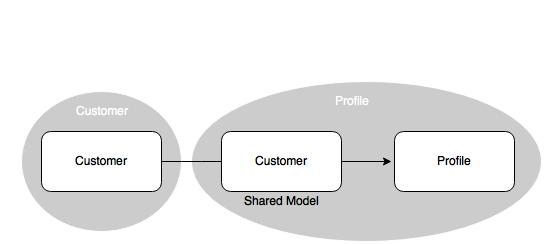
\includegraphics[width=0.8\textwidth]{figures/domain-driven-design-two}
\caption{Domain Model for Customer Management}
\label{fig:domain_driven_design/example_scenario/subdomains/Customer}
\end{center}
\end{figure}
\\
The management of customer includes two distinct broad task which are managing the customer itself and management of attributes of each customer which contribute to creating profile of customer at any point of time. Although, these two functionalities are related to customer, are actually loosely coupled and have different performance requirement. For eg: the change in the decision of adding attribute to a customer profile does not change the way customer is managed and also the rate at which customer profile is updated will definitely have high value than the rate customer is managed. Additionally, not all the attributes from customer is relevant to customer profile which makes 'Customer' a polyseme and a shared model between the two bounded contexts 'Customer' and 'Profile'.\\

\begin{shaded} Booking \end{shaded}
\\
\begin{figure}[H]
\begin{center}
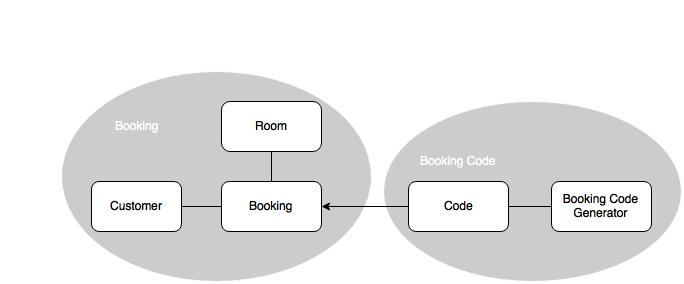
\includegraphics[width=0.8\textwidth]{figures/domain-driven-design-three}
\caption{Domain Model for Booking}
\label{fig:domain_driven_design/example_scenario/subdomains/booking}
\end{center}
\end{figure}
\\
The Figure \ref{fig:domain_driven_design/example_scenario/subdomains/booking} shows the domain models of "Booking" subdomain. All the domain models and terms inside the subdomain are consistent and clear. However, the models 'Room', 'Customer', 'Booking' and 'Code' are closely related to booking functionality whereas the functionality of generating the booking code can be considered independent of booking. This gives two loosely coupled bounded contexts: "Booking" and "Booking Code". It is also interesting to notice that the models 'Customer' and 'Room' are polysemes with regard to other 'Customer' and 'Room' bounded contexts.\\
\begin{shaded} Checkout \end{shaded}
\\
\begin{figure}[H]
\begin{center}
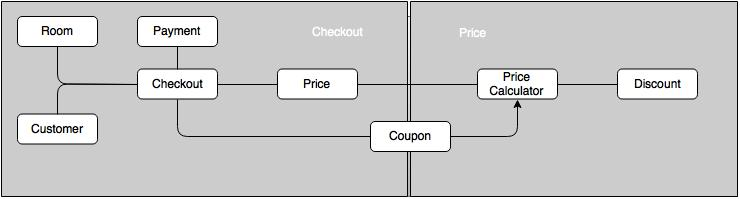
\includegraphics[width=0.8\textwidth]{figures/domain-driven-design-four}
\caption{Domain Model for Checkout}
\label{fig:domain_driven_design/example_scenario/subdomains/checkout}
\end{center}
\end{figure}
\\
The overall billing price calculation during checkout, which includes validation of coupon and redeem of the coupon onto the total price, is independent of the orchestration logic which occurs during checkout. The subdomain can be realized into two different bounded contexts 'Checkout' and 'Price'. Additionally, the domain models 'Customer, 'Discount', 'Room', 'coupon' and 'price' are polysemes for these bounded context with respect to other bounded contexts.\\
\begin{shaded} Package Management \end{shaded}
\\
\begin{figure}[H]
\begin{center}
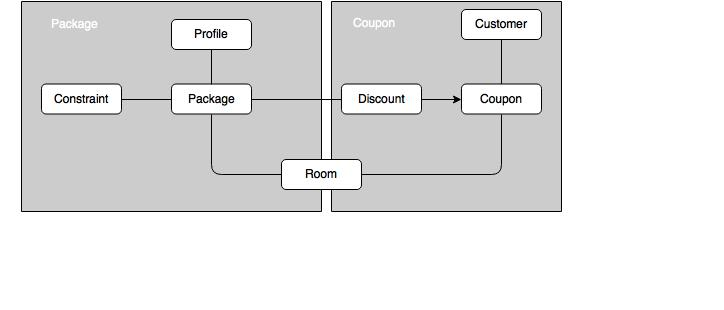
\includegraphics[width=0.8\textwidth]{figures/domain-driven-design-five}
\caption{Domain Model for Package Management}
\label{fig:domain_driven_design/example_scenario/subdomains/package-management}
\end{center}
\end{figure}
\\
The logic of package management can be considered independent of the way coupon is generated and validated. The packages are created by staff memeber whereas a coupon is created upon receiving a request from customer. Additionally, these are very specific and independent responsibilities, eligible of having own bounded contexts. The only data shared by the bounded contexts are about the information regarding eligible rooms and discount values. It should be made clear at this point that the 'Profile' domain model here is very different than 'Profile' domain model from 'Profile' boundend context of 'Customer Management' subdomain. In here, 'Profile' model defines the attributes of generic customer eligible for a specific package, however the 'Profile' domain model in 'Profile' bounded context provides the updated characteristics of any individual customer at the moment. Similarly, the models such as 'Customer' and 'Room' are polysemes.\\
The same process can be applied to identify bounded contexts for rest of the subdomains.

\section{Conclusion}\label{section:modeling_microservices/conclusion}
The use case refactoring process discussed in Section \ref{section:selection_by_use_case/use_case} highlights an important concept regarding use cases fulfilling multiple cross-cutting concerns and thus provides solutions by breaking down these concerns into individual use case modules, each focused on cohesive tasks. This kind of decomposition truely relates to the characteristics of microservices. On the other hand, domain driven design technique presented in Section \ref{section:domain_driven_design/introduction} provides a different approach of understanding the problem domain well using ubiquitous language, dividing the big problem domain into multiple manageable sub-domains and then finally using the concept of bounded context to determine individual microservices. The microservices thus obtained are autonomous and focus on single responsibility.\\
The use case refactoring process utilizes use cases as its modeling tool, which is not only easy but the familiar tool to architects and developers. This makes use case refactoring a faster approach to decompose a problem domain. Whereas, domain driven design has ubiquitous language and bounded context at its core. Both of these concepts are complex and new to most architects as well as developers. At the same time, understanding problem domain correctly at the first attempt is rare and it will take quite a few iterations to get the decomposition right. Thus, domain driven design is not the faster approach of modeling microservices.\\
Visualizing a problem domain in terms of diferent use cases seems like a natural way but dividing a big problem domain into smaller independent manageable sub-domains as stated by domain driven desing, can be a smart way to decompose. So, in case of big and complex problem domain, it can be very difficult to visualize in terms of large number of big use case trees and task trees. This may lead to microservices without appropriate level of granularity and quality attributes.\\
A good thing about use case refactoring is that it provides very easy way to break down use case along various level of functionalites or abstraction. However, it undermines another crucial concept which is data ownership and data decompostion. An explicit assumption is made about an entity model being a single source of truth for whole domain, but it is rarely true. Using this approach will not necessarily produce autonomous services. However, the concept of ubiquitous lanugage and bounded context used by domain driven design, highly focus on different and unique local representation of same entity. This highly favors the autonomy of the resulting microservices. At the same time, the bounded context are responsible for small sets of cohesive functionality. This adheres to single responsibility principle. Thus, bounded context represents the appropriate size for a microservice.

\section{Problem Statement}\label{section:modeling_microservices/problem_statement}
It is interesting to understand the various strategies defined in the literature to decompose a problem domain into microservices. The concept of microservices architecture is getting very popular recently among a lot of industries. So, the understanding of the process used in industries can also add bigger value to the thesis. For this reason, the next step is to study architecture at SAP Hybris as well as the process it followed for modeling microservices to build its commerce platform.


